%%%%%%%%%%%%%%%%%%%%%%%%%%%%%%%%%%%%
% This is the template for submission to ISCA 2017
% The cls file is a modified from  'sig-alternate.cls'
%%%%%%%%%%%%%%%%%%%%%%%%%%%%%%%%%%%%

%\documentclass{sig-alternate} 
\documentclass[journal]{IEEEtran}
\usepackage{mathptmx} % This is Times font
%\newcommand{\ignore}[1]{}
\usepackage{fancyhdr}
\usepackage[normalem]{ulem}
\usepackage[hyphens]{url}
\usepackage{hyperref}
\usepackage{epsfig}
\usepackage{multirow}

%%%%%%%%%%%---SETME-----%%%%%%%%%%%%%
%\newcommand{\iscasubmissionnumber}{461}
%%%%%%%%%%%%%%%%%%%%%%%%%%%%%%%%%%%%

%\fancypagestyle{firstpage}{
%	\fancyhf{}
%	\setlength{\headheight}{50pt}
%	\renewcommand{\headrulewidth}{0pt}
%	\fancyhead[C]{\normalsize{ISCA 2017 Submission
%			\textbf{\#\iscasubmissionnumber} \\ Confidential Draft: DO NOT DISTRIBUTE}} 
%	\pagenumbering{arabic}
%}  

% This package is used to write algorithms (see Buchberger's algorithm
% in the text). File algorithm2e.sty included in the directory
\usepackage[ruled]{algorithm2e}
%%for algorithm2e package, label has to be following caption in the same line!!!
\renewcommand{\algorithmcfname}{ALGORITHM}
\SetAlFnt{\small}
\SetAlCapFnt{\small}
\SetAlCapNameFnt{\small}
\SetAlCapHSkip{0pt}
\IncMargin{-\parindent}


% These packages will help you with Math and Figures
\usepackage{helvet}
\usepackage{enumerate}
\usepackage{amsmath}
\usepackage{amsfonts}
\usepackage{graphicx}
\usepackage{multirow}
\usepackage{subfig}
\usepackage{comment}
\usepackage{mathtools}
%\usepackage{algorithm}
%%indent in algorithm

\setcounter{page}{1}


% New command for the table notes.
\def\tabnote#1{{\small{#1}}}
% New command for the line spacing.
\newtheorem{Algorithm}{Algorithm}[section]
%\newtheorem{Definition}{Definition}[section]
%\newtheorem{Example}{Example}[section]
%\newtheorem{Proposition}{Proposition}[section]
%\newtheorem{Lemma}{Lemma}[section]
%\newtheorem{Theorem}{Theorem}[section]
%\newtheorem{Corollary}{Corollary}[section]
%\newtheorem{Proof}{Proof}


%%% These are my macros that I use for math symbols
\newcommand{\B}{{\mathbb{B}}}
\newcommand{\Z}{{\mathbb{Z}}}
\newcommand{\R}{{\mathbb{R}}}
\newcommand{\Q}{{\mathbb{Q}}}
\newcommand{\N}{{\mathbb{N}}}
\newcommand{\C}{{\mathbb{C}}}
\newcommand{\Zn}{{\mathbb{Z}}_{n}}
\newcommand{\Zp}{{\mathbb{Z}}_{p}}
\newcommand{\F}{{\mathbb{F}}}
\newcommand{\Fbar}{{\overline{\mathbb{F}}}}
\newcommand{\Fq}{{\mathbb{F}}_{q}}
\newcommand{\Fqbar}{{\overline{{\mathbb{F}}_q}}}
\newcommand{\Fkk}{{\mathbb{F}}_{2^k}}
\newcommand{\Zkk}{{\mathbb{Z}}_{2^k}}
\newcommand{\Fkkx}[1][x]{\ensuremath{\mathbb{F}}_{2^k}[#1]\xspace}
\newcommand{\Grobner}{Gr\"{o}bner\xspace}
\newcommand{\bi}{\begin{itemize}}
	\newcommand{\ei}{\end{itemize}}
\newcommand{\idealj}{{J = \langle f_1, \dots, f_s\rangle}}
\newcommand{\idealg}{{J = \langle g_1, \dots, g_t\rangle}}
\newcommand{\vfqj}{{V_{\Fq}(J)}}


%Page header

%%%%%%%%%%%---SETME-----%%%%%%%%%%%%%

%\title{Implementation of Bitcoin Hash using SHA-256 algorithm}
%\author{Vikas Kumar Rao, Yomi Karthik Rupesh, Rajath Bindiganavile, Sreejita Saha \\
%	Department of  Electrical and Computer Engineering\\
%	University of Utah, Salt Lake City, UT-84112\\\{vikas.k.rao,yomikarthik.rupesh,\}@utah.edu }
%\maketitle

%%%%%%%%%%%%%%%%%%%%%%%%%%%%%%%%%%%%
\begin{document}
\markboth{Bitcoin hashing using SHA-256}{Prof. Kalla is the best}
\title{Implementation of Bitcoin Hash using SHA-256} 
\author{Vikas Kumar Rao, Yomi Karthik Rupesh, Rajath Bindiganavile, Sreejita Saha \\
	Department of  Electrical and Computer Engineering\\
	University of Utah, Salt Lake City, UT-84112\\\{vikas.k.rao,yomikarthik.rupesh,Rajath.bindiganavile,sreejita.saha\}@utah.edu}
\maketitle
%\maketitle
%s\thispagestyle{firstpage}

%\pagestyle{plain}
\begin{abstract}

Resolving an unknown component is a fundamental problem encountered in
post-verification debugging and automatic correction of digital
circuits. Contemporary techniques rely on iterative/incremental
application of SAT solving and Craig interpolation to realize the
functionality of (or resolve) the unknown components. While these
techniques have achieved some success for control-dominated
applications (random logic circuits), they are infeasible in resolving
the unknown components in arithmetic circuits. This paper describes an
algebraic approach to resolve the functionality of an unknown
component in a finite field arithmetic circuit so that the circuit
implementation matches a given specification. Starting from an
equivalence checking setup modeled as a polynomial ideal
membership test in commutative algebra, we formulate the problem of
resolving the unknown component as a quantification procedure. Using
the \Grobner basis algorithm, we derive an approach to identify the
function implemented by the unknown component. We go on to pose the
problem as a synthesis challenge and explore the space of polynomial
functions for the unknown component by analyzing quotients of
ideals. As \Grobner basis algorithms exhibit high computational
complexity, we exploit the circuit topology to improve our
algorithms. We can resolve the unknown components not just for
bit-level circuit implementations, but also in cases where the
abstraction hierarchy is given at the level of (bit-vector)
words. Experiments performed over various finite field arithmetic
circuits demonstrate the efficacy and superiority of our approach as
compared to conventional techniques.

  % Resolving an unknown component is a fundamental problem encountered
  % in logic synthesis for engineering change orders, post-verification
  % debugging and automatic correction of digital circuits. Contemporary
  % techniques rely on the iterative/incremental application of SAT solving
  % and Craig interpolation to realize the functionality of (or resolve)
  % the unknown components. While these techniques have achieved some
  % success for control-dominated applications (random logic circuits),
  % they are infeasible in resolving the unknown components in
  % arithmetic circuits. This paper describes an algebraic approach to
  % resolve the functionality of an unknown component in an arithmetic
  % circuit so that the circuit implementation matches a given
  % specification. Our approach is formulated as a polynomial ideal
  % membership test. We go on to pose the problem as a synthesis
  % challenge and explore the solution space of the unknown component
  % using concepts from the quotient of ideals. We propose a \Grobner basis 
  % based algorithm for a systematic, goal driven search for
  % implementable solutions. The paper presents results on some
  % experiments performed over various finite field arithmetic circuits
  % to compare the efficiency of our approach against recent methods.   


% Automatic bug correction is a tedious and resource intensive process. 
%% Automatic correction of unknown components in a given circuit is a
%% resource intensive process. Recent developments in realizing the
%% functionality implemented by these unknown gates rely on incremental
%% SAT solving. Despite using state-of-the-art SAT solvers, these
%% approaches fail to verify multipliers beyond 12-bits and hence are
%% infeasible in a practical setting. The current formal datapath
%% verification methods which utilize symbolic computer algebra concepts,
%% rely heavily on textbook structure of the circuits to realize an
%% unknown component, and hence are not scalable. These approaches model
%% circuit as a set of polynomials over integer rings, and use function
%% extraction, simulation, and term rewriting using coefficient
%% computation to arrive at a solution. The approach is not complete in
%% the sense that the procedure cannot be extended to random logic
%% circuits and finite field circuits due to ambiguities in coefficient
%% computation. The approach also fails to verify circuits when redundant
%% gates are introduced in the design. To overcome all these limitations,
%% this paper describes a formal approach using finite field theory to
%% automatically realize the function implemented by an unknown
%% component, and verify the same. The paper introduces theory on
%% resolving a single unknown component using ideal membership testing
%% and \Grobner basis based reduction. We go onto pose the problem as a
%% synthesis challenge and extend the solution space of the unknown
%% component using concepts from quotient of ideals. Since the solution
%% space is not unique, we will also discuss a systematic, goal driven
%% search for simple implementable solutions. The paper presents results
%% on some preliminary experiments performed over various arithmetic
%% circuits to compare efficiency of our approach against recent methods.  
\end{abstract}

%\section{Introduction}
Verifying functional correctness of gate-level arithmetic circuits is still a significant challenge owing to ever increasing design size and functional complexity. A considerable amount of manual intervention is required to localize a bug and correct it, thus making it a resource intensive process. Traditional automated debugging techniques based on simulation, decision procedures such as Binary Decision Diagrams (BDDs)~\cite{bryant:1} and SAT solvers~\cite{alanmi:2006} demand bit-blasting of the circuit, and are hence considered inefficient models to verify complex datapath designs. Due to the inherent algebraic nature of computations in such designs, symbolic algebra algorithms are considered more appropriate for their verification.

Under symbolic algebra environment, a given specification and its circuit implementation are modeled as a set of polynomials. The verification problem is then formulated as \textit{membership testing}~\cite{gb_book} which can prove/disprove whether the circuit implements the specification. In the case of buggy circuits the verification fails; faulty gate(s) are identified and a correction is computed to rectify the circuit. The paper considers a single gate fault model i.e., exactly one of the gates in the circuit is incorrectly synthesized thereby implementing a wrong function at its output. For example, an AND gate replaced with an XOR gate. Once a particular gate has been identified as buggy, we label this gate as the \textit{unknown component}. We propose an approach to realize a correction function which can be implemented at the output of this \textit{unknown component}, such that the entire circuit implementation conforms to the specification. Identifying the buggy gate in a given circuit implementation is a much harder problem and is in the future scope of our work. This paper puts forth the underlying theory on realizing and exploring the solution space for correction functions, and outlines the future verification challenges.
\vspace{-0.1in}
\subsection{Previous work}

The most recent and relevant approach~\cite{fujita:2015},~\cite{fujita:2012} resolves the unknown component problem using an incremental $SAT$ formulation. The paper models the unknown component in a given circuit($Ckt$) as a LUT by using transformation variables($X$). The solution to these variables implements the desired logic function so that the resulting circuit becomes logically equivalent to a given specification $Spec()$. Let $Ckt(X,In)$ be the formula corresponding to the given circuit with possible transformations, where $In$ is the set of all primary inputs to the circuit. This can be formulated naturally as a two-level QBF with a existential quantifier followed by a universal quantifier as shown below:
\vspace{0.1in}
\begin{align}
\exists \textit{X}.\forall \textit{In. Ckt(X,In) = Spec(In)}:    
\end{align}

The two level QBF is then solved by repeatedly applying the below SAT formulation:
  
\begin{enumerate}
	\item Let Target=($Ckt(X,In)\neq spec(In))$. Let $k$ be the num-ber of test vectors, initialized to zero. Let $TestSet$ be the set of all generated test patterns, initialized to the empty set.
	\item Check if Target is satisfiable.
	\item If SAT, $k=k+1$ and record the solution as $TestSet = TestSet \cup in_k$. The Target is then updated as Target = (Target($X,In))\land(Ckt(X,in_k)=Spec(in_k))$, and go to step 2.
    \item If UNSAT, we have all the required test set patterns $\{in_1$ $\dots in_k\}$. Now, check if: $(Ckt(X,in_1) = Spec(in_1)) \land (Ckt(X,in_2) = Spec(in_2)) \land \dots (Ckt(X,in_k) = Spec$ $(in_k))$ is satisfiable.
    \item If SAT, then any solution $X$ is a correct set of transformation, while an UNSAT result proves that there does not exist a correct set of transformation.
\end{enumerate}

% By experiment, the approach shows that if the circuit is correct under these input patterns($in_k$), it is guaranteed to be correct for all of $2^{In}$ input patterns.
The work in~\cite{maciej:2017} poses the unknown component formulation as a camouflaged circuit model and tries to de-obfuscate several types of camouflaging techniques using incremental SAT solving. The approach used in~\cite{andreas:2005} inserts logic corrector MUXs on the unknown sub-circuits and relies on SAT solvers to realize the functionality. 

Despite using state-of-the-art SAT solvers, all the above approaches fail to verify large and complex finite field arithmetic circuits. The solvers still model the problem as decision procedures and, as demonstrated by our experimental results, are shown to be inefficient in solving verification problems on multiplier circuits beyond 12-bits. 

The technique from Farahmandi et al.~\cite{farimah:2016} deals with automatic debugging and correction using computer algebra concepts. The authors use function extraction~\cite{maciej:2015:1} with a specific term order~\cite{lv} to do equivalence checking, subsequently generating a remainder in case of failure. The approach then finds all possible assignments to variables of the remainder such that it generates a non-zero value. This test set helps arrive at a pruned gate list for bug localization. The procedure then takes every gate in the pruned list, starting from primary inputs, and tries to match the appeared remainders pattern. It does so by computing the difference between the polynomial computed at the output of the suspicious gate against the polynomial computed by a probable set of gate corrections. The coefficient computation~\cite{maciej:2015:2} during pattern matching relies heavily on the half-adder based circuit structure. The paper doesn't discuss the ambiguities in weight calculations when the gate structure differs from the given topology. The approach is not complete in the case when there are redundant gates in the circuit as we found through our experiments. The approach also doesn't talk about finite field arithmetic circuits as the experiments are illustrated with only integer arithmetic circuits.

% and hence The approach also fails to arrive at a conclusive solution when the circuit is tweaked with some redundancy and hence lacks completeness. 

% While theorem provers require extensive manual intervention and expertise. 

% Additional constraint relating floating signals to fanouts in the circuit must be satisfied for the result to be trusted; however the computation to verify this condition can be expensive. For this reason, this method becomes inefficient if the number of logic gates dominates the HA network. Also, the circuit would need to be partitioned into linear and non-linear portions, which is a non-trivial task.

% \subsection{Contribution}
% % by extending it to random logic circuits. 
% The paper discusses a single gate replacement error model as the target design i.e., only one gate in the design incorrectly replaced, for example an AND gate replaced with an XOR/OR gate. We are given a circuit implementation $C$, modeled as a set of polynomials $F=\{f_1,\dots,f_s\}$, with one of these gates $f_i$ marked as unknown component. We then utilize concepts from symbolic computer algebra to realize the function implemented by this unknown component. The reference golden model can either be a specification polynomial $f$ or a different circuit $C_1$ implementing the same function as circuit $C$. For a given specification polynomial $f$, we do polynomial reduction until the unknown component gate and arrive at the function implemented by the component by using \Grobner basis based guided ideal membership testing, and elimination ideal. For the case where the specification is given in terms of a different implementation $C_1$, we use \Grobner basis based reduction on a miter setup to arrive at a solution. %, and apply $\it{Nullstellensatz}$ principles to verify the function implemented by the component%
% This paper seeks to put forth the underlying theory, outline the verification challenges, and present a complete approach to resolve an unknown component in finite field arithmetic circuits. We also discuss some preliminary but encouraging experimental results and draw a comparison to the SAT-based approach.  

% The paper will address both the notions by analyzing the circuit polynomials using concepts from computer algebra\cite{gb_book}\cite{ideals:book} such as \Grobner basis reduction, projection of variety, elimination ideal, ideal membership testing, and weak $\it{Nullstellensatz}$.

%Extra
% Partial synthesis required for logic optimization and Engineering Change Order(ECO). Design is treated as a combinatorial black box, and in order to determine the logic function realized by the design, it is necessary to constraint the circuit topologically. A set of sub-circuits considered as vacant with fixed inputs are treated used for transformation to realize the function implemented by the unknown component.
\section{Introduction}
\label{section:background}
Bitcoin is an upcoming and growing form of digital currency which does not require the conventional third parties like banks for transactions. Bitcoin allows an easy peer-to-peer transaction network where a person can directly pay another person without reverting to trusted parties like banks.

The transactions that are through these third parties like banks can take some number of days to complete as well as require some transaction fees. Hence the emergence of cryptocurrency proved to be beneficial. Bitcoin is however the first cryptocurrency that established a completely trustless transaction network where there is no trsust between the two parties involved in a transaction.

The bitcoin network is based on Cryptographic proof, and takes advantage of public key cryptography. Fig. 1 explains the method of working of the bitcoin network explicitly. If Vikas wants to send a bitcoin to Yomi, Yomi sends his address to Vikas. When Vikas is sending a bitcoin to Yomi, the private key of Vikas is used for encryption to send the bitcoin, which serves as a digital signature of Vikas. However to authenticate the validity of this transaction, the recipients of the bitcoin will require the public key of Vikas. The public key of Yomi also gets added to the bitcoin and it gets broadcasted throughout the bitcoin network letting everyone in the network know that the particular bitcoin now belongs to Yomi. Similar transactions form a series and gets broadcasted in form of block chain throughout the network. 

The bitcoin network is a decentralized network and does not have a singular centralised authority to check if the transactions are valid or not. Thus there could be instances of double spending where a person might send the same bitcoins to two people and it would be not possible to assess who the actual recipient of the bitcoins is. Thus the transaction block needs to be validated. To ensure the validity, a "proof of work" function needs to be added to each block.

Bitcoin miners contribute computation power to the network to verify the authenticity of the transactions and add these blocks to the existing block chain. Bitcoin miners generally have ASICs built to serve the function of this mining. Presently whenever a bitcoin transaction block is validated the miner is given some number of bitcoins as a mining reward. This is done to motivate bitcoin users to secure transactions and also distribute bitcoins in a decentralized way. Bitcoin mining is perfectly parallel meaning that many bitcoin hashes can be computed simultaneously on separate cores without any communication between the cores.  Bitcoin can potentially serve as a payment method worldwide without reverting to the discrepancies of different currencies. Our aim is to implement one such fast and easy-to-mine bitcoin hash generating ASIC, with a good hash rate.

\begin{figure}[ht]
	\begin{center}
		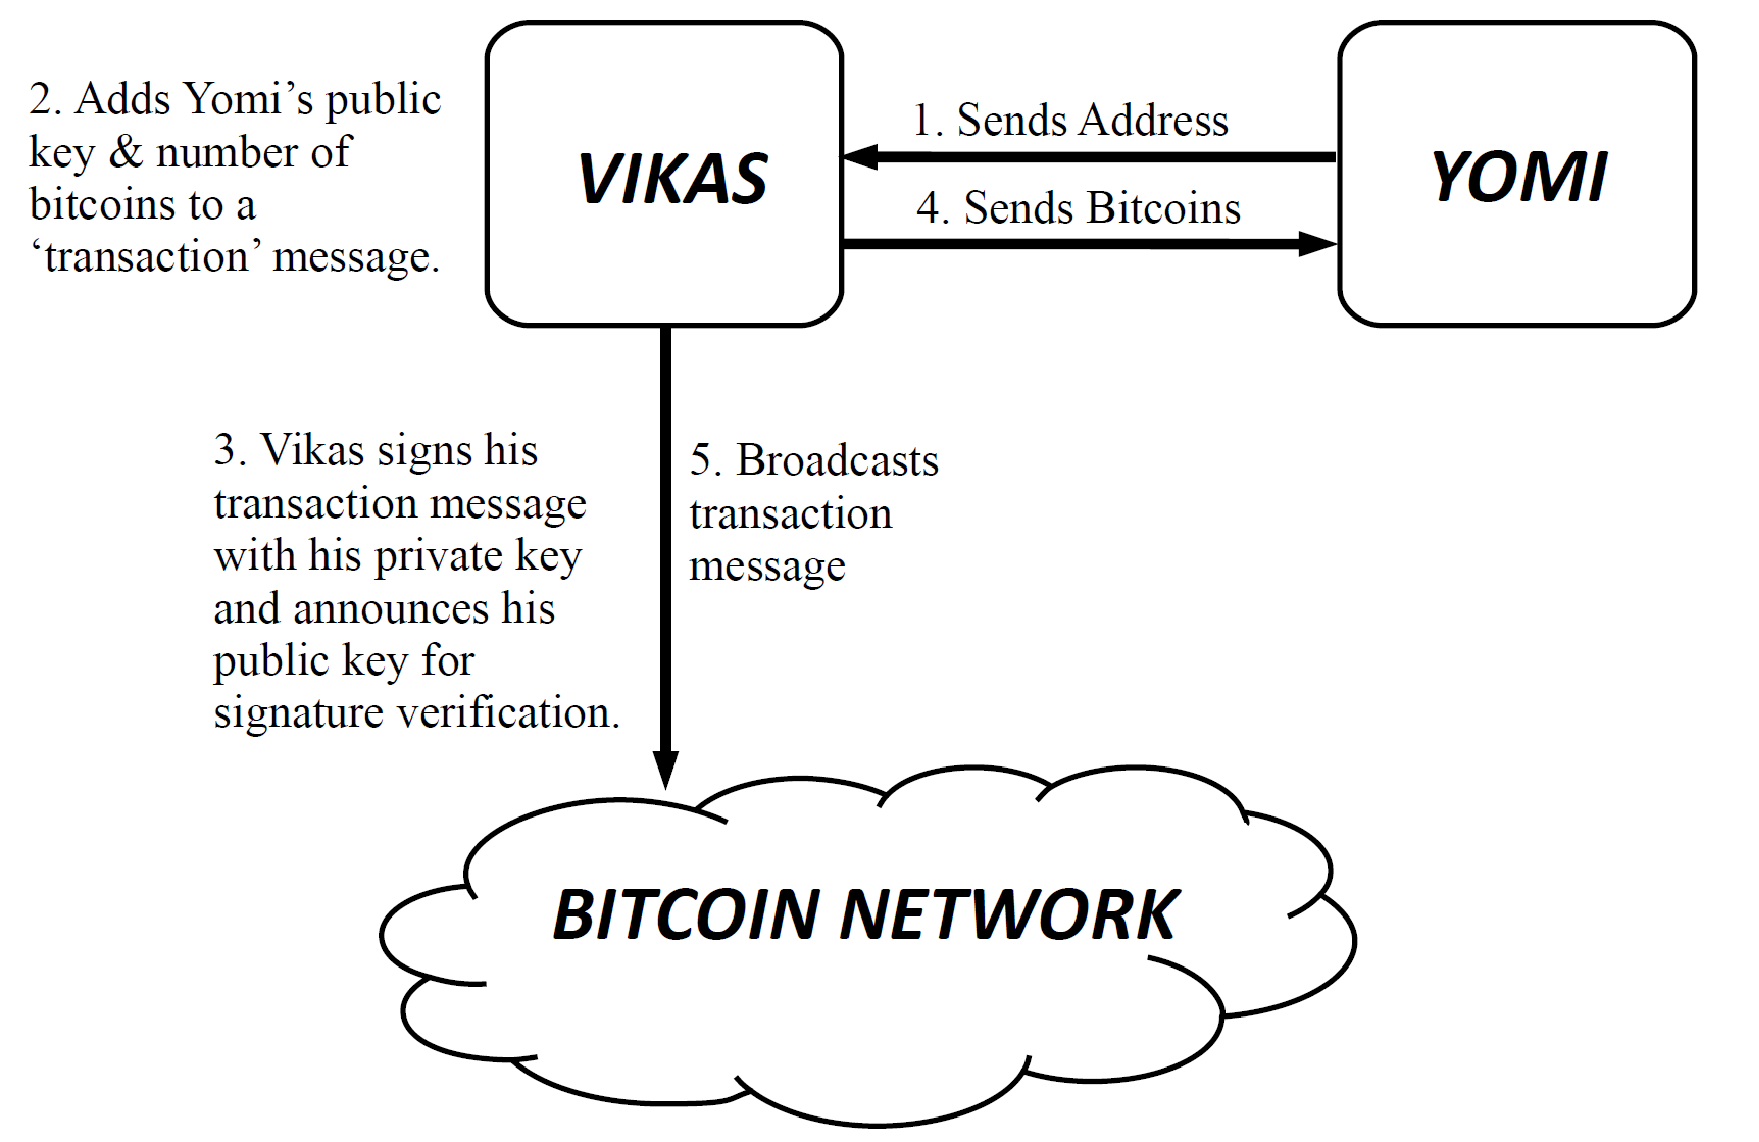
\epsfig{file=Figures/bitcoin_network.pdf, width = \columnwidth}
	\end{center}
	\vspace{-1ex}
	\caption{ Working model of Bitcoin Network 
		\label{Working of Bitcoin Network}}
	\vspace{-4ex}
\end{figure}

\section{Motivation and Scope of the Project}
When a block is getting validated over the network, a protection mechanism is used so that no illegal blocks can be added to these transactions by any form of malicious attempt. A proof of work function is added to each block to ensure its validity. Hashcash is such a proof of work function that is used by bitcoin network and it uses two iterations of SHA-256 algorithm ~\cite{SHA-256}for it's implementation. Just like any other hash function it encrypts data of any arbitrary size into a fixed sized data. If even one bit of the input data is modified, it generates a completely different hash value.
However, bitcoin theft has been documented on several
occasions. There were instances when the bitcoin exchanges
have shut down taking the client’s bitcoins with them. It is
thus extremely important for a strong encryption algorithm to
secure the bitcoin framework. Of late many leading organi-
zations have started accepting bitcoins and it has started to
appeal to general masses as well. Hence bitcoin miners are an integral part of the bitcoin community and is critical to the survival and security of the bitcoin network. Their willingness to contribute their computational power to secure transactions are thus rewarded by the bitcoin community. We were hence motivated to implement our own ASIC that could potentially append transactions in the bitcoin network with a good hash rate.   
Eventhough, the ASIC implementation is capable of mining bitcoins, our focus is to implement the hascash function with a pre-defined block\_header.

\begin{algorithm}[hbt]
	
	{
	block\_header = \{ Version + prev\_block + merkle\_root + timestamp + bits \} \\
			nonce = 0, 	hash = 1\\
	target = 0.000123456789\\
	\While{(\textbf{hash} $>$ \textbf{target})}{hash = SHA256(SHA256(nonce + block\_header))
		\\nonce++}
	}
	\caption {Simplification of mining algorithm}
	\label{mining}
\end{algorithm}

\section{Block Header Fields}
Algorithm Table~\ref{mining} depicts the mining algorithm~\cite{FPGA} involved in bitcoin hashing.
The algorithm shown includes several keywords which are as follows: \\
Version - The version of the block. \\
Prev\_block - Hash value of the previous block. \\
Merkle\_root - hash value of the merkle root of the current block i.e,hash value of the transactions in the current block. \\
Timestamp - current time in seconds after 1970-01-01 T 00:00 UTC. \\
Bits - Number of bits of nonce used to meet the target.


\section{Design Approach}
The core design implementation in the project is of the encryption algorithm SHA-256  Figure~\ref{SHAblockdiagram}, which consists of message packing, scheduling, constant storage, and core math compression. Based on the traditional approach for implementation of the compression technique, we are estimating a gate count close to 120,000 per compression block. The total area over a $0.6\mu$m process technology is being approximated at $0.6nm^2$~\cite{area1,area2}. 


\subsection{Message padding and parsing}
Let's consider a message $M$ of length $L$ bits as input. The message is appended with bit '1' at the end of the message and the resulting data is padded with '$k$' number of 0's, where '$k$' is the smallest non-negative solution to satisfy $k=448-(L+1)$. The message is padded with zero's until the length of message becomes $448\%512$. The rest $64$ bits is length of the message 'L' appended as a 64-bit binary number, thus resulting in a $512$ bit block. If the message is greater than 55 characters, the spillovers form a new $512$ bit message block. Thus the message M is composed into $N$ $512$ bit blocks which are each denoted by $M(1), M(2), M(3) ... M(N)$. 

\begin{figure}[ht]
	\begin{center}
		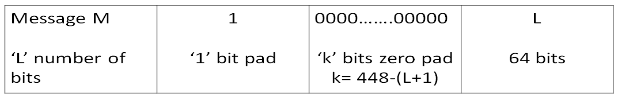
\epsfig{file=Figures/block.png, width = \columnwidth}
	\end{center}
	\vspace{-1ex}
	\caption{A typical padded message 
		\label{padded message}}
	\vspace{-4ex}
\end{figure}

\begin{figure}[ht]
	\begin{center}
		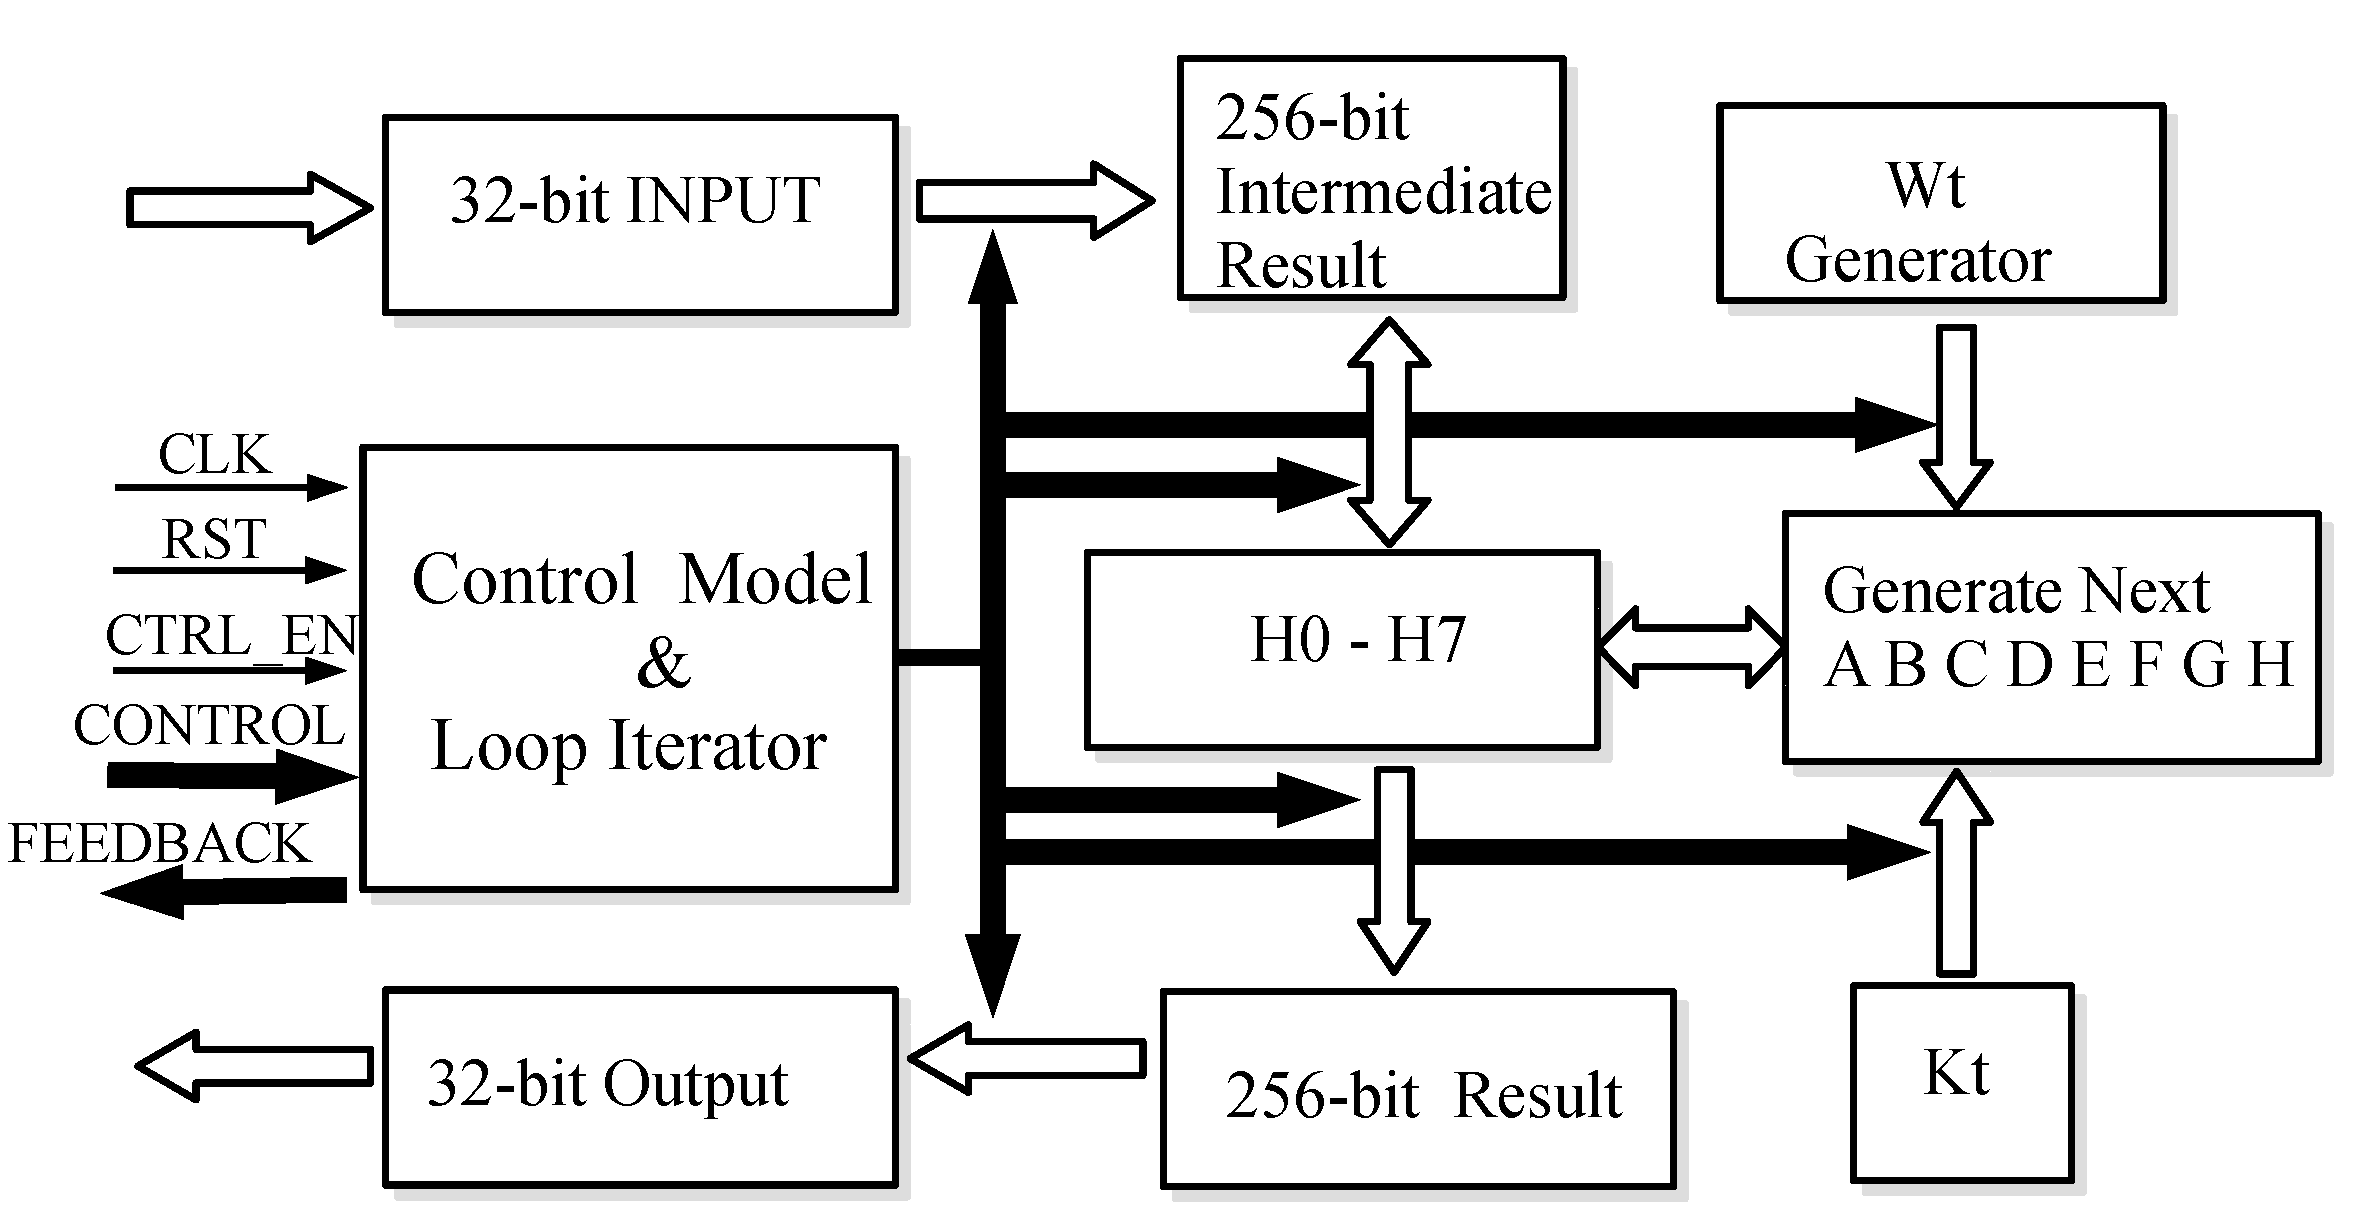
\epsfig{file=Figures/SHA-256.pdf, width = \columnwidth}
	\end{center}
	\vspace{-1ex}
	\caption{Block Diagram of SHA-256. 
		\label{SHAblockdiagram}}
	\vspace{-4ex}
\end{figure}


\subsection{Message expansion, constants, and scheduling}
Each of the $512$ bit $M(i)$ blocks are broken down into 16 32-bit blocks $M_{t}(i)$, where $0 \leq t \leq 15$. The message expansion results in each 512 bit block to get expanded into 64 32-bit blocks denoted by $W(t)$, where $0 \leq t \leq 63$. The message expansion takes place in SHA-256 algorithm using the following set of operations~\cite{FPGA}:

$\sigma_{0} (x) = ROT_{7}(x) \oplus ROT_{18}(x) \oplus SHF_{3}(x) $

$\sigma_{1}(x) = ROT_{17}(x) \oplus ROT_{19}(x) \oplus SHF_{10}(x)$
 
$W_{t} = \begin{cases} 
	M_{t}(i), 0 \leq t \leq 15 \\
	\sigma_{1}(W_{t} - 2) + W_{t} − 7 + \sigma_{0}(W_{t} − 15) + W_{t}-16, 16 \leq t \leq 63  
\end{cases}$

$ROT_{n}(x)$ is a circular rotation of x by n positions to the right.

$SHF_{n}(x)$ is a right shift of x by n positions. 

The expansion also involves pre-defined constants published by NIST. The scheduling involves streaming 32-bit word as input to the subsequent stages of SHA-256 compression.
\begin{figure}[ht]
	\begin{center}
		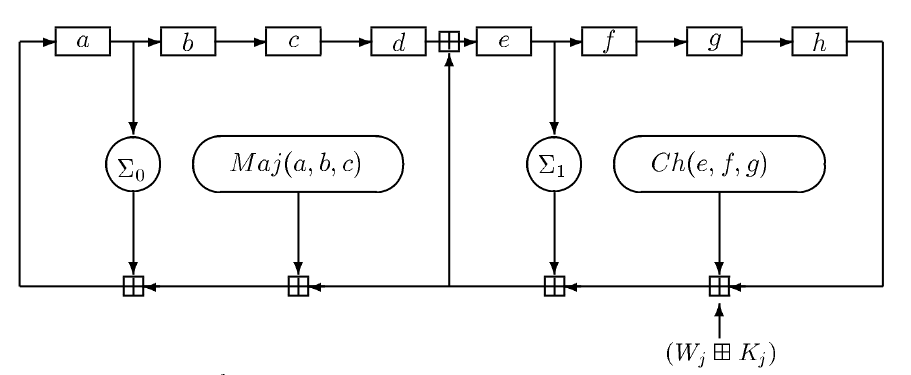
\epsfig{file=Figures/M2.png, width = \columnwidth}
	\end{center}
	\vspace{-1ex}
	\caption{Message Scheduling 
		\label{Message Scheduling}}
	\vspace{-4ex} ~\cite{SHA-256}
\end{figure}
\subsection{Core message Compression}
SHA-256 compression function works on the streamed $W(t)$ block that we get from the expansion stage. In totality, the SHA-256 compression function is computed over a loop on the 512 bit message blocks as follows ~\cite{Newcastle}

$H(i) = H(i-1) + CM(i)(H(i-1))$

Where, C is the SHA-256 compression function.
'+' is word wise mod  $2^{32}$ addition
$H(i)$ is the hash value that is generated for the message $M(i)$.

The compression function uses 8 32-bit variables \textit{A, B, C,.... H}. These are the initial constant values for the first loop of compression and are initialized to the first 32 bits of the fractional parts of the square roots of the first eight prime numbers.~\cite{FPGA} We actually use our block header and encrypt these eight constants. This compression is iterated 64 times using the following operations:

$T_{1} = H + \sum_{1}(E)+ Ch(E,F,G) + K_{t} + W_{t}$

$T_{2} = \sum_{0}(A) + Maj(A,B,C)$
\\where
\\$Ch(x,y,z) = (x AND y) \oplus (\bar{x} AND z)
\\Maj(x,y,z) = (x AND y) \oplus (x AND z) \oplus (y AND z)
\\\sum_{0}(x)= ROT_{2}(x) \oplus ROT_{13}(x) \oplus ROT_{22}(x)
\\\sum_{1}(x)= ROT_{6}(x) \oplus ROT_{11}(x) \oplus ROT_{25}(x)$~~\cite{FPGA}\\The $K_{t}$ inputs are 64 32-bit constants which are initialized to the first 32 bits of the fractional parts of the cube roots of the first 64 prime numbers. \cite{FPGA}
\begin{figure}[ht]
	\begin{center}
		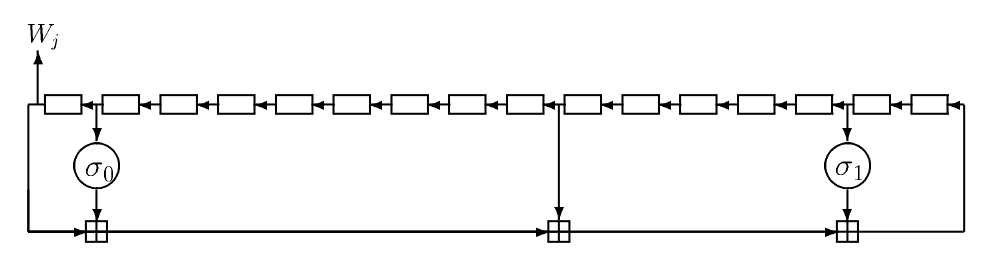
\epsfig{file=Figures/M1.png, width = \columnwidth}
	\end{center}
	\vspace{-1ex}
	\caption{Message Compression
		\label{Message Compression}}
	\vspace{-4ex} ~\cite{SHA-256}
\end{figure}
\\During every $i^{th}$ iteration, $ \\ H=G\\ F=E\\ D=C\\ B=A\\G=F\\E=D+T_{1}\\C=B\\ A= T_{1}+T_{2}$~\cite{FPGA}
\\After 64 iterations of this SHA-256 compression function the immediate hash values are computed. 
\\$H_{0}^{(i)} = A + H_{0}^{(i-1)}$
\\$H_{1}^{(i)} = B + H_{1}^{(i-1)}$
\\$H_{2}^{(i)} = C + H_{2}^{(i-1)}$
\\$H_{3}^{(i)} = D + H_{3}^{(i-1)}$
\\$H_{4}^{(i)} = E + H_{4}^{(i-1)}$
\\$H_{5}^{(i)} = F + H_{5}^{(i-1)}$
\\$H_{6}^{(i)} = G + H_{6}^{(i-1)}$
\\$H_{7}^{(i)} = H + H_{7}^{(i-1)}$ \cite{FPGA}
\\This compression algorithm is computed on all the 512-bit blocks. Suppose there are $N$ 512-bit blocks, the final 256-bit hash output is the concatenation of the hash values of $N^{th}$ block.
\\$H^{N} = H_{0}^{(N)}H_{1}^{(N)}H_{2}^{(N)}H_{3}^{(N)}H_{4}^{(N)}H_{5}^{(N)}H_{6}^{(N)}H_{7}^{(N)} $ \cite{FPGA}


\subsection{Overview of Bitcoin mining implementation}
The block header is used to encrypt the constants specified by NIST. Our block header consists of 640 bits- Version[31:0], Previous hash value[255:0], Merkle Tree [255:0], Timestamp[31:0], Difficulty bits [31:0], Nonce[31:0].
\\Bitcoin mining requires finding the value of the cryptographic nonce so that the hash value is within a certain range for that block. The nonce value is such that the double SHA-256 hash value of the block is less than a given $threshold$ value. This $threshold$ value varies over time as a function of the difficulty bits that is adjusted by the network itself such that a valid transaction block is added to the network approximately every ten minutes. This means that a valid hash of hash solution, that matches the given $threshold$, is found every ten minutes. The first miner who finds the valid nonce value broadcasts it throughout the bitcoin network and is thus rewarded. 
\\Nonce is the last 32 bits of the block header. As mentioned earlier the nonce value needs to be changed until the double hash of the block meets the given threshold, thus nonce is the only changing bits in the entire 640 bits block header.Out of these 640 bits, the first 512 bits do not need padding as these bits are fixed for a particular hash computation. These bits can itself form the first 512-bit block and can directly continue to the parsing stage. The rest 128 bits of the 640-bit header are padded to produce the second 512-bit block. The first 512 bits do not change across nonce iterations hence it's hash can be precomputed. This 256-bit hash value of the first block is parsed into 8 32-bit values and are used to encrypt the second block instead of the the given $A, B, C,....H$ values. The hash output of the second block is hashed again using SHA-256 which gives the final hash value. This final hash value is checked against the $threshold$.
\\The constituent core blocks (Figure ~\ref{ourimplementation}) are developed in verilog HDL with each operation register size being 32 bit DWORD. Every RTL core is validated through a individual verilog testbench to get a block level debug view. The final top level test bench has our module implementation output compared against a SHA-256 software model implementation. All the necessary basic cells and gates for the project is taken from those developed in the group project library. 

\begin{figure}[ht]
	\begin{center}
		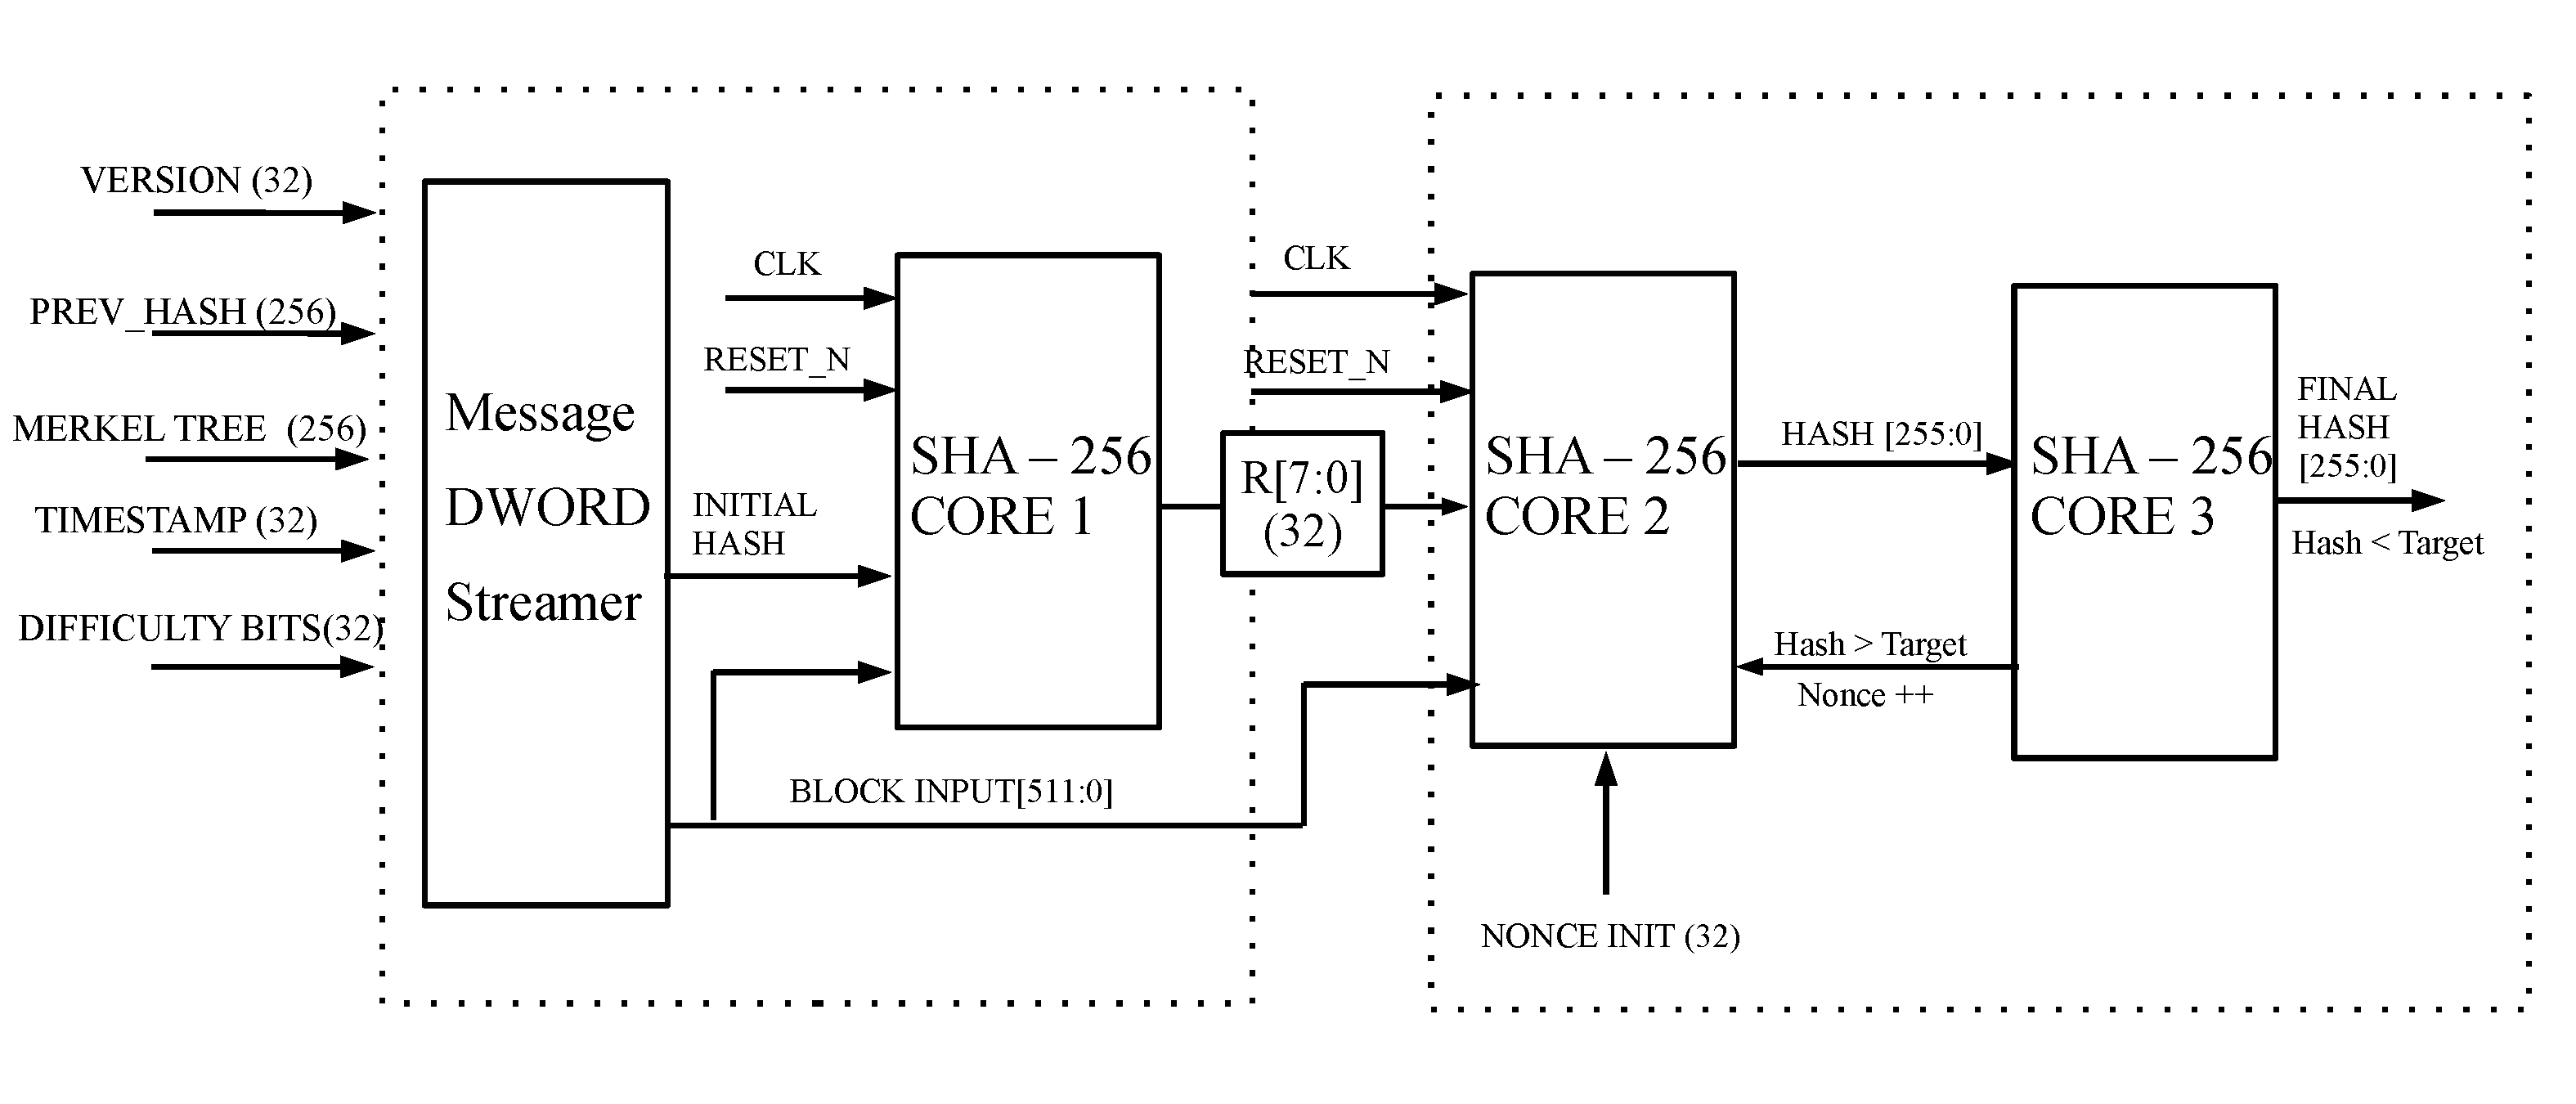
\epsfig{file=Figures/bitcoin.pdf, width = \columnwidth}
	\end{center}
	\vspace{-2ex}
	\caption{Our Bitcoin Implementation. 
		\label{ourimplementation}}
	\vspace{-2ex}
\end{figure}

To reduce the layout area imprint for block operations, we have also developed some hand-written, optimized DWORD gates. 


\section{ASIC Implementation}
Our ASIC is implemented using Verilog and synthesized using Synopsys Design Compiler. The development of the ASIC core involved building RTL cores for the every function implementation which are then verified using individual verilog testbenches.
\subsection{RTL Approach}
We define two cores for our Verilog design, one of which performs iterations and the other core to carry out all our ALU computations. 
\\The SHA-256 expansion stage performs two different types of operations based on the value of $t$ which is the the value of the iteration as discussed earlier. The $Iterator$ core that we designed takes 32-bit message input $M{t}(i)$ from the parsing stage and computes $W_{t}$. The value of $W_{t}$ remains the same as the input $M{t}(i)$ for the first 16 iterations that is for $t$ ranging from 0 to 15. The $W_{t}$ for $t$ values ranging from 16 to 63, is computed using rotating and shifting functions on the previous $W_{t}$ values generated for every iteration. Our $Iterator$ core uses $genvar$ for implementation of these two $for$ loops.$Genvar$ is a variable used in generate-for loop in verilog and stores positive integer values. The $Iterator$ calls functions that are defined in our $ALU$ core.
\\The second core that performs ALU operations defines separate modules for each functional operation. This core computes the values of $ \sigma_{0}, \sigma_{1}, Maj, Ch $ functions. It basically performs the Rotation, Shifting, XOR, AND operations required for those functions. These operations are called from the $Iterator$ core. Thus the functions defined here in the $ALU$ core are used in the $Iterator$ core for each iteration in the SHA-256 Algorithm.
\subsection{Testbench Approach}
Each of our RTL cores are validated using Verilog testbenches to get a debug view of each and every stage of the SHA-256 Algorithm and also the entire Bitcoin mining double hash. Our testbench has a block header input, checks first the 256-bit hash computed for that block with the actual hash value for that block. This validates a single working SHA-256 hash core that we implemented. A testbench also checks the double hash for a 640-bit block header with a working software implementation of a bitcoin hash generator.
We checked if our SHA-256 core is working by using several input block headers. As an example, if our input message to the SHA-256 core given is $abc$, we get the hash of this input as: \\ba7816bf 8f01cfea 414140de 5dae2223 b00361a3 96177a9c b410ff61 f20015ad
\\We verified this output through a testbench with the actual SHA-256 hash of $abc$.
This computation of hash involved multiple steps. At the first, each of a, b and c was converted into their 8-bit ASCII value.
\\8 bit ASCII of a: 01100001
\\8 bit ASCII of b: 01100010
\\8 bit ASCII of c: 01100011
This 24 bit word was now padded with a '1' and 423 '0's followed by '24' in a 64 bit binary. The resulting padded message was thus 512 bits.This 512-bit message was broken down into 16 32-bit DWORDS which were then expanded to form 64 32-bit DWORDS using message expansion as discussed above. The expanded message is then compressed using the SHA-256 compression function, thus producing the hash value.
Once we verified the working of one SHA-256 core, our double hash digest was also verified using the testbench.
\section{Hardware Implementation} 
The bitcoin mining double hash that we implemented using behavioral verilog was synthesized using the library that we built. This library consists of basic cells AND, AOI, 4X\_Buffer, 8X\_Buffer, Ch function(Choosing) , D- FLIPFLOP, Filler cell, Inverter, 4X\_Inverter, 8X\_Inverter, Maj function(Majority), NAND, 2X\_NAND, NOR, TIEHIGH, TIELOW, XOR, XNOR.
\\The library was first characterized using the Signal Storm Tool in Cadence to generate the $.db$ file and the Abstract tool was used to generate a $.lef$ file. This $.db$ file was used in Synopsys Design Compiler to synthesize the structural verilog code from the behavioral verilog code. We performed place and route using the synthesized verilog file and the generated $.lef$ file with a row spacing of 60 microns and density of 10\%. Due to large amount of parallel operations and hence greater number of wires, there were many violations.To reduce these violations occurring from congestion, we prevented the tool from flipping the cells that it does to reduce area. Finally this was taken back to Virtuoso for Design rule and Schematic checks. This resulted in an ASIC having an area of XX and a gate count of XX with yy AND, yy AOI, 4X\_Buffer, 8X\_Buffer, Ch function(Choosing) , D- FLIPFLOP, Filler cell, Inverter, 4X\_Inverter, 8X\_Inverter, Maj function(Majority), NAND, 2X\_NAND, NOR, TIEHIGH, TIELOW, XOR, XNOR.
\section{Results}
\section{Further Optimizations Proposed}
After having read and reviewed research papers based on Bitcoin mining and SHA-256, we intend to incorporate the optimizations explicitly stated in those papers to enhance our implementation of a bitcoin hash ASIC. 
\\~\cite{} mentions that bitcoin mining is a suitable candidate for approximate computing. The parallel nature of bitcoin mining can be exploited to increase bitcoin mining profits by replacing circuits with their approximate versions and allowing a Better than Worst-Case (BTWC) operation. Approximations give greater mining profits even when the hash computed is incorrect, as any wrong solution gets invalidated by other bitcoin miners in the network. This optimization trades off reliabity with delay and area. Using approximate circuits reduces delay which in turn increases frequency and overall throughput. It also reduces area, which can be used for incorporating more hashing cores on the ASIC. From the results reviewed from the paper it is seen that there's a 30\% increase in mining profits using approximate adder $KSA_{16}$(Kogge Stone Adder) compared to their accurate counterparts like $CLA$ (Carry-lookahead adder) or $KSA_{32}$. 15\% of the 30\% increased profit is due to functional approximation that is using approximate cirtuits and the other 15\% is derived from operational approximation. Operational approximation involves reducing guard bands, running the cicuit at a negative timing slack, BTWC operation and allowing ocassional timing violations. We plan to try and design the $KSA_{16}$ adder for out bitcoin miner in order to increase mining profits.  

\section{Conclusion}

%\input{fade}
%\input{cache}
%\input{dram}
%\section{Experimental Setup}
\label{section:setup}

%We evaluate the area, frequency, and power overheads of DESC by implementing it in Verilog HDL, and synthesizing the proposed hardware.
%
We evaluate the area, frequency, and power overheads of FADE-Basic, FADE-LLC, and FADE-DDR by synthesizing the proposed hardware. To assess the energy and performance potentials of FADE-DDR, we use CACTI IO~\cite{CACTI,jouppi2015cacti}, Micron power calculator~\cite{micron-ddr,micron-lpddr}, and DRAMPower~\cite{chandrasekar2012drampower}. We simulate 14 memory-intensive parallel applications as well as 5 sequential SPEC2006 applications, running on a heavily modified version of the ESESC simulator~\cite{ESESC}.
Using McPAT~\cite{McPat}, we estimate the overall processor power.

\subsection{Design Space Exploration}
A modified version of CACTI 6.5~\cite{CACTI} is used to find the best suitable configuration for L2 and L3 caches for full swing interconnects, as well as FADE-Basic and FADE-LLC interfaces. The cache sizes of L2 and L3 are fixed to 256KB and 8MB respectively and the number of banks is fixed to 8. Design space for full swing wires (64 wires) is explored by varying between ITRS high performance(HP), ITRS low standby power(LSTP) and ITRS low power(LOP) devices~\cite{NUCA}, whereas for FADE-Basic (76 wires) and FADE-LLC (80 wires) interfacess, a range of reduced voltages are applied on ITRS-HP, ITRS-LSTP and ITRS-LOP to find the most energy efficient peripheral circuitry for the SRAM cells. We scale the delay of low power wires, making use of delay model illustrated in ~\cite{scalingfactor}. Energy metric Energy Delay Product~\cite{edp} is used to determine the most energy efficient configuration.

\subsection{Methodology}
Besides FADE, we evaluate and compare other existing encoding techniques such as Bus invert coding~\cite{bus-invert}, DESC~\cite{desc}, BD encoding~\cite{bdencoding} and CAFO~\cite{CAFO}. These encoding techniques are evaluated against conventional binary encoding. Similar to FADE, for a single core system we apply all the encoding techniques only to the last level cache, whereas for multi core system we apply it to both L2 and L3. Conventional binary encoding with both normal and reduced voltages are applied to DDR interface and cache. Reduced voltage conventional binary encoding includes utilization of low power wires at cache level and LPDDR3 as DRAM technology. Bus invert coding is applied to cache levels while data bus invert is applied to the DDR interface. DESC is applied only to the cache levels as it restricts its application to DDR interface due to varying burst lengths. BD encoding exploits data similarity in cache block and reduces number of ones and bit flips. A 64 and 32 entry recent data table is opted for DDR interface and cache respectively for BD encoding. A smaller entry size is chosen for cache due to the large area overhead introduced by a 64 size entry table. CAFO, a two dimensional DBI technique, is applied to both DDR interface and cache levels.

\subsection{Architecture}
We modify the ESESC simulator~\cite{ESESC} to model a multicore and a single core computer systems.
The multicore system comprises four OoO cores with private L1 and L2 caches and a shared 8MB LLC, interfaces to two DDR4-3200 DRAM channels.
The single core system consists of two cache levels, interfaced with a DDR4-3200 DRAM channel.
Table~\ref{table:para} shows the simulation parameters.

\begin{table}[h!]
	\centerline{
		{\scriptsize\begin{tabular}{|c|c|c|}
				\hline
				& \textbf{Multithreaded} & \textbf{Single-threaded} \\
				\hline
				& four 4-issue OoO cores,    & a 4-issue OoO core, \\
				\textbf{Core}       	 & 128 ROB entries,    & 128 ROB entries,  \\
												& 3.2 GHz        & 3.2 GHz  \\
				\hline
				& 32KB, 4-way, LRU, & 32KB, 4-way, LRU, \\
				\textbf{IL1/DL1 cache}   & 64B block,           & 64B block, \\
				\textbf{(per core)}  & hit/miss delay 2/2   & hit/miss delay 2/2 \\
				\hline
				& 256KB, 8-way, LRU,     & 8MB, 8-way, LRU, \\
				\textbf{L2 cache}   & 64B block,           & 64B block, \\
				\textbf{(per core)}  & hit/miss delay 2/5,  & hit/miss delay 10/5, \\
				& MESI protocol        & MESI protocol \\
				\hline
				\textbf{L3 cache}    & 8MB, 8-way, LRU, 64B block, & -- \\
				\textbf{(shared)}    & hit/miss delay 10/5 & -- \\
				\hline
				\textbf{Temperature} & \multicolumn{2}{c|}{$350\,^{\circ}{\rm K}$ ($77\,^{\circ}{\rm C}$)} \\
				\hline
				\textbf{DRAM}        & 2 DDR4-3200, FR-FCFS & 1 DDR4-3200, FR-FCFS \\
				\hline
		\end{tabular}}
	}
	\vspace{-1ex}
	\caption{Simulation parameters.\label{table:para}}
	\vspace{-1ex}
\end{table}

%cache: (1) a Niagara-like eight-core processor, and (2) a single-threaded out-of-order processor.
%Both systems have an 8MB L2 cache, interfaced to two DDR3-1066 DRAM channels.
%
%FADE is assessed on L1 cache size of 32KB, L2 of 1 MB and L3 of 8MB. In case of a single core, the last level cache is L2 with 8MB size. A two channel DDR system is used with LPDDR3's unterminated interface. Caches of very large size has a major impact on the energy dissipated by it. There is a lot of leakage energy in SRAM cells and peripheral circuitry that needs to be optimized. Apart from increased power consumption in case of large caches, there is a huge impact on performance. Because of its large size, it takes several additional cycles to fetch a cache block.
%
%A sensitivity study to explore the design space of L2 and L3 caches is carried out using CACTI 6.5. This study results in the most energy efficient system configuration with respect to both SRAM cells and its peripheral circuitry. For both L2 and L3, the design space is explored for various bank counts alongside a variation in the output width. A wide range of ITRS High performance wires(HP), ITRS low power (LOP) and ITRS low standby power(LSTP), without altering their threshold voltages is considered in the design exploration to achieve an energy efficient system. The results show that using a LSTP technology for cell type and LOP for peripheral  resulted in a configuration with minimal performance degradation and power consumption. The most energy efficient cache configuration for L2 and L3 is achieved for 8 banks with 64 wires. High performance wires are used for L1 cache as it is very sensitive to delays.  

%ESESC is modified to incorporate conventional binary encoding technique, bus-invert coding~\cite{bus-invert}, BD encoding~\cite{bdencoding}, CAFO~\cite{CAFO} and FADE for both cache and DRAM interface. Also, DESC~\cite{desc} is included for only cache. The number of segments for bus invert coding is decided based on a sensitivity test, to find out the best value for number of segments, as bus invert coding is sensitive to the segments. Zero skipping is included in DESC, which further brings down the number of transitions in this scheme. 

\subsection{Applications}
A mix of 14 parallel benchmarks from Phoenix, SPALSH-2~\cite{Splash2}, and NAS~\cite{NAS} suites is used to evaluate the impact of FADE codes on memory intensive benchmarks.
The valuated single threaded applications are from SPEC2006~\cite{spec2006} suite running on the single core processor.
Table~\ref{table:applications} summarizes the evaluated benchmarks and their input sets.
%All the applications (Table~\ref{applications}) are run on ESESC with the necessary input files.

\begin{table}[h!]
	\vspace{-1.5ex}
	\centerline
	{\scriptsize\setlength\tabcolsep{1.5pt}
		\begin{tabular}{|c|c|c|c|}
			\hline
			&\textbf{Benchmarks}  & \textbf{Suite} &\textbf{Input} \\
			\hline
			\parbox[t]{2mm}{\multirow{14}{*}{\rotatebox[origin=c]{90}{\textbf{Parallel}}}}
			& Linear Regression & Phoenix &  100MB key file \\
			& Matrix Multiplication  & Phoenix & Matrix length = 1000 \\
		    & Parallel Cache Assignment & Phoenix & 1000x 2000 matrix\\
		    & Rindex & Phoenix &  \\ 
		  	& String Match & Phoenix & 500MB key file  \\ 
		  	& Wordcount & Phoenix & 100MB word text file  \\ 
		  	& kmeans & Phoenix & 3 Dimension-1000 each,\\
		  	& & &  points =100000\\ 
		  	\cline{2-4}
		   	& Fourier Transform & NAS OpenMP & Class A \\ 
		   	& Integer Sort & NAS OpenMP & Class A \\ 
		   	& Multi-Grid on a sequence of meshes & NAS OpenMP & Class A \\ 
		  	& Conjugate Gradient & NAS OpenMP & Class A \\ 
		  	\cline{2-4}
		   	& Radix & SPLASH-2 & 2M integers \\ 
		  	& Ocean-C & SPLASH-2 & 514x514 ocean \\ 
		   	& Cholesky & SPLASH-2 & tk29.0 \\ 
		    \hline
		    \parbox[t]{2mm}{\multirow{5}{*}{\rotatebox[origin=c]{90}{\textbf{Single-threaded}}}}
		     & BZip2 & SPECint 2006 & reference \\
		    & Hmmer & SPECint 2006 & reference \\ 
		    & MCF & SPECint 2006 & reference \\
		    \cline{2-4} 
		    & Lattice Boltzmann Method & SPECfp 2006 & reference \\ 
		    & Simplex Linear Program (LP) Solver & SPECfp 2006 & reference  \\ 
		    & & & \\
		    \hline    
		   \end{tabular}
	}
	\vspace{-1.5ex}
	\caption{Application and data sets.\label{table:applications}}
	\vspace{-1.5ex}
\end{table}

%Dimension-3 each 1000, cluster- 100, points =100000 
%~\hspace{-\normalbaselineskip}
\subsection{Synthesis}
The area, delay, and power for the FADE encoders and decoders are based on FreePDK~\cite{FreePDK45} at 45nm, which are then scaled to 22nm using~\cite{45nmto22nm1,45nmto22nm2}.
% Table~\ref{synthesis}. The encoders and decoders for both the cache and DDR is designed to have minimal area overhead.

%\begin{table}[h!]
%	\vspace{-1.5ex}
%	\centerline
%	{\scriptsize\setlength\tabcolsep{1.5pt}
%		\begin{tabular}{|c|c|c|}
%			\hline
%			\textbf{Technology}  & \textbf{Voltage} &\textbf{FO4 Delay} \\
%			\hline
%			45nm & 1.1 V & 20.25ps \\
%			22nm & 0.83 V & 11.75ps \\
%			\hline    
%		\end{tabular}
%	}
%	\vspace{-1.5ex}
%	\caption{Technology Parameters.\label{synthesis}}
%	\vspace{-1.5ex}
%\end{table}

%\input{evaluation}
%\section{Related Work}
\label{section:related}
Numerous existing ideas for cache energy and memory interface optimizations have been studied. Various factors contribute to the overall energy dissipation for both on-chip and off-chip communication.Every factor has a considerable impact on the energy consumption, thus requiring optimization for every such factor.  
 
\subsection{Energy Efficient Data Encoding Techniques}
Dynamic energy is dependent on frequency, load capacitance, voltage and activity factor. The average transitions that occur during one clock cycle, is accounted by activity factor. Every transition on the interconnects consumes energy and it is required to reduce the number of transitions in every cycle in order to reduce dynamic energy. Data encoding techniques, have been formed in the past, which reduce the activity factor, hence bringing down the dynamic energy.

Transitions occur for every change in the data bits, hence it is important to limit the Hamming weight of codewords. 3 Limited weight codes (3-LWC) is an example of M-LWC encoding scheme~\cite{limitedweight}, where the codewords have a Hamming weight of no more than M. These codewords, bring about a major reduction in the dynamic energy consumed as the Hamming weight and thus the transitions occurring due to the codewords reduces. In 3-LWC encoding scheme, one byte of data is transferred with a codeword which is 17bits long and with a maximum of three ones. A table storing all the frequently transferred data~\cite{frequentencoding} can be used. Every time data needs to be sent, it looks in to the table. When the data to be sent, is found in the table, a simple codeword with hamming distance of 1 is sent over an extra wire. This is an energy efficient scheme, when the frequency of similar data is high. In case, the data cannot be found in the look up table, the original data is sent over the wires.

When a data block needs to be transferred, an XOR operation is performed with previously transmitted data block~\cite{XORencoding}. This operation exploits the temporal locality between continuous blocks of data. An XOR operation of the present data with the previously transferred one, checks the difference in data between consecutive blocks and thus reduces transitions per clock cycle.  

Flip-N-Write~\cite{flipnwrite}, encodes the data to be written in either the original form or in its inverted form. A comparison is done with the previously stored data and accordingly picks the the form of data to be used. It is an extension of BI coding~\cite{bus-invert}, which improves the write energy in phase change memory. A write operation is modified into a read before write operation, in order to only transfer contradicting bits over the wire. 

    
\subsection{Memory Interface Optimizations}
DRAM data bus contributes a significant portion of the processor energy. Prior works to reduce the data transfer energy on the DRAM data bus have been discussed in this section. BD-encoding~\cite{bdencoding} compares the data to be sent over the DRAM data bus, with data which was sent over it recently. Based on the similarity with prior stored data set, the encoding scheme decides whether to send the xor-ed data i.e., original data xor-ed with most similar recent data word or to send the original data word. \cite{CAFO}, uses a cost calculating scheme, with respect to the number of transitions. A positive gain, leads to inversion of the bits. Data bus invert coding scheme is applied to both rows and columns, until no further reduction of bit flips is possible. More is Less~\cite{moreisless}, is another work to reduce the energy dissipated over the DDR data bus. This work exploits the inactive nature of the data bus due to timing constraints within the DRAM. A longer codeword with less ones, which utilizes the data bus for a longer time is used, in order to reduce the energy used for data transfer. All these techniques focus on reducing the number of ones/zeros to be transferred to reduce the termination energy. FADE-DDR completely removes termination energy by switching to unterminated interface and further reduces switching energy by employing efficient encoding for low swing transisitional signalling. An extension of bus invert~\cite{bus-invert}  is data bus invert~\cite{dbi}, where the number of 1s are checked for the present data rather than with the previous data.     



\subsection{Cache Energy Optimizations}
In the past, various encoding schemes have been presented for cache energy optimization. Bus invert coding~\cite{bus-invert}  is an energy efficient bus encoding technique, where Hamming distance of the data to be sent and  previously sent is calculated. If the Hamming distance exceeds N/2 for an N bit data, all the N bits need to be inverted. This encoding technique forms segments of bits, in order to use an extra wire for every segment. Bus invert is sensitive to the segment number and needs to be chosen carefully. The extra wire is used to indicate whether the data transmitted is either in original or inverted form by a bit-0 or bit-1 respectively. 
DESC~\cite{desc} employs a time dependent transfer scheme using synchronized counters. DESC is applicable only to the last-level cache and doesn't reduce the interconnect energy for upper levels. Reducing data movement energy via online data and clustering encoding, talks about reducing the number of transitions over the last level cache and the DDR interface. This is done with the help of clustering, where the data that needs to be transmitted chooses the clustering centers with least hamming distance and performs an XOR with the original data. The data transmitted includes the residual information and additional bits, to identify the cluster center at the receiver end. Every time a data has been transmitted, the cluster is updated both at the transmitter and the receiver end.
DESC~\cite{desc} is a time-dependent encoding scheme to transmit information over wires. Data to be transferred is divided into groups of 4-bits(chunks) representing a value range from 0-15. Based on the value 'N' represented by the chunks, a bit flip is introduced after 'N' clock cycles of transmission of the previous chunk. This technique includes a reset line to initiate a data transfer. In addition to the conventional encoding, this techniques includes additional schemes such as zero skipping and last value skipping, which further reduce the flips required for transmission of the data.




  

%\input{conclusions}


%%%%%%% -- PAPER CONTENT ENDS -- %%%%%%%%

%%%%%%%%% -- BIB STYLE AND FILE -- %%%%%%%%
\bibliographystyle{ieeetr}
\bibliography{ref}
%%%%%%%%%%%%%%%%%%%%%%%%%%%%%%%%%%%%

\end{document}
